\level{1}{Pianificazione}
	Si è deciso di dividere lo sviluppo del progetto in varie fasi. Il termine di ognuna di esse è segnato da una milestone. Una milestone può essere o una scadenza di consegna di revisione o un incontro con il proponente. Si è preferito fissare milestone non a lunga distanza tra loro per ridurre i rischi e permettere di aver un resoconto da parte del proponente ad ogni fase. Per ogni fase di sviluppo vengono pianificati vari periodi di verifica per ogni attività, solitamente uno ogni 7 giorni con durata media di 2 giorni. Ogni verifica è importante perché quella diventerà una baseline.\\
	Il periodo di svolgimento del progetto è quindi stato diviso nelle seguenti fasi:
	\begin{description}
		\item[Fase DB (Documentation Beginning):] Questa fase è caratterizzata da 3 sottofasi:
			\begin{itemize}
				\item individuazione/creazione degli strumenti per documentazione e di supporto;
				\item creazione \insdoc{Norme di Progetto};
				\item creazione documentazione (\insdoc{Studio di Fattibilità}, seguito da \insdoc{Analisi dei Requisiti}, \insdoc{Piano di Progetto}, \insdoc{Piano di Qualifica} e \insdoc{Glossario}).
			\end{itemize}
			In questa fase l'attività più onerosa sarà quella di analisi.\\Tra la seconda e la terza sottofase viene effettuato un incontro con il proponente per chiarire le idee sulla comprensione del capitolato.\\Tale fase si conclude con la \insrev{Revisione dei Requisiti}. In tale modo si avrà un riscontro immediato sulle intenzioni del proponente.
		\item[Fase DI (Documentation Improvement):] Caratterizzata dall’analisi di dettaglio. In questa fase verranno consolidati i requisiti  e verrà portato un incremento o una correzione a tutti i documenti scritti fino ad ora, se necessario.\\Tale fase si conclude con un incontro con il proponente che visionerà e confermerà le modifiche fatte al documento \insdoc{Analisi dei Requisiti}.
		\item[Fase SD (Software Design):] Caratterizzata dalla progettazione architetturale. Questa fase ha inizio quando il documento \insdoc{Analisi dei Requisiti} è nello stato tra \textit{acceptable} e \textit{addressed} (fine \insphase{Fase DI}) e termina con la visione del proponente. Verranno apportati incrementi ad alcuni documenti prodotti nelle precedenti fasi, come \insdoc{Norme di Progetto}, \insdoc{Piano di Progetto}, \insdoc{Glossario} e \insdoc{Piano di Qualifica}. Al proponente si prevede di mostrare il documento \insdoc{Specifica Tecnica}.
		\item[Fase P (Prototyping):] In questa fase si procede con la progettazione di dettaglio e la codifica dei requisiti obbligatori. Tale fase si conclude con la visione del proponente di un primo prototipo che dovrà soddisfare i requisiti obbligatori e la scadenza della consegna per la \insrev{Revisione di Progettazione}. Verranno apportati incrementi ai documenti prodotti nelle precedenti fasi. Alla revisione si prevede di consegnare il documento \insdoc{Specifica Tecnica} steso fino a quel momento ma non la progettazione al dettaglio dei requisiti obbligatori che verrà consegnata per la \insrev{RQ} insieme al resto.
		\item[Fase IP (Increase of the Prototype):] Avrà inizio subito dopo la scadenza della consegna per la \insrev{Revisione di Progettazione}. In questa fase si procede con la progettazione di dettaglio e la codifica dei requisiti desiderabili. Tale fase si conclude con la visione del proponente di un secondo prototipo che dovrà soddisfare i requisiti obbligatori e desiderabili. Verranno apportati incrementi ai documenti prodotti nelle precedenti fasi.
		\item[Fase CP (Completion of the Product):] Avrà inizio subito dopo la consegna per la \insphase{Fase IP}. In questa fase si procede con la progettazione di dettaglio e la codifica dei requisiti opzionali. Tale fase si conclude con l'incontro con il proponente per mostrare il prototipo con tutti i requisiti implementati e con la scadenza della consegna per la \insrev{Revisione di Qualifica}. Verranno apportati incrementi ai documenti prodotti nelle precedenti fasi. Si prevede quindi di consegnare le ultime versioni dei documenti ed il documento \insdoc{Definizione di Prodotto} completo di tutta la progettazione al dettaglio ed il codice.
		\item[Fase PD (Product Delivery):] Tale fase comincia non appena termina la \insphase{Fase CP}. Essa è caratterizzata dalla validazione e quindi il lavoro più oneroso sarà quello dei \insrole{verificatori}. In questa fase il progetto avrà termine. Verrà quindi effettuata la validazione del software creato e successivamente verrà collaudato. Tale fase si conclude con la \insrev{RA}.
	\end{description}
	La scelta effettuata ci permette di spezzare facilmente ognuna di queste 7 macro-fasi in attività più piccole. Questo permette di avere maggior controllo sull'avanzamento del progetto, e soprattutto dà la possibilità di applicare il PDCA molto frequentemente.\\Ad ognuna delle varie attività sono state associate una o più risorse. Delle sotto-attività è stato riportato unicamente il Gantt.\\ 
	Di seguito saranno elencate le durate e le caratteristiche di ogni fase. I tempi sono stati pensati per permettere uno slack sufficiente per abbassare i rischi relativi alle tempistiche.
	% !TEX encoding = UTF-8 Unicode
\level{2}{Fase DB: Documentation Beginning}
	\textbf{Periodo}: dal \insdate{25}{11}{2014} al \insdate{23}{01}{2015} \\
	Questa fase comincia con la presentazione in aula delle “regole del progetto didattico”. Essa termina con la scadenza della consegna della \insrev{Revisione Dei Requisiti}.\\Le sottofasi sono le seguenti:
	\begin{description}
		\item[Individuazione/creazione strumenti:] In questa sottofase vengono scelti gli strumenti che saranno utilizzati per la stesura dei documenti, per il tracciamento dei requisiti e alcuni script di controllo dei documenti. Se alcuni di essi non sono disponibili nella rete o non soddisfacenti, verranno creati su misura.
		\item[Norme Di Progetto:] Dopo aver individuato gli strumenti si potrà procedere alla stesura del documento \insfile{Norme di Progetto v1.00}. Questo documento sarà utilizzato indipendentemente dal capitolato che sarà preso in appalto.
		\item[Creazione documentazione:] In questa fase sappiamo esattamente con cosa e in che modo dobbiamo scrivere un documento e possiamo iniziare la stesura dei documenti.
			\begin{itemize}
				\item \textbf{Studio Di Fattibilità}: Vengono valutati pro e contro di tutti i capitolati proposti e viene redatto il documento \insdoc{Studio di Fattibilità v1.00}. Viene quindi scelto il capitolato da sviluppare.
				\item \textbf{Analisi Dei Requisiti}: Viene steso il documento \insdoc{Analisi dei Requisiti v1.00}. Prima e durante la stesura di questo documento verranno fatti degli incontri con il proponente per consolidare i requisiti stesi o per chiarire le idee sui requisiti da stendere.
				\item \textbf{Piano Di Progetto}: Si stende il documento \insdoc{Piano di Progetto v1.00} per regolare le attività che il team dovrà svolgere.
				\item \textbf{Piano Di Qualifica}: Si redige il documento \insdoc{Piano di Qualifica v1.00}.
				\item \textbf{Glossario}: viene incrementato il file  \insfile{Glossario.xml} e steso in modo automatico il documento \insdoc{Glossario v1.00}.
			\end{itemize}
	\end{description}
	\level{3}{Diagramma di Gantt delle attività}
	\begin{figure}[H]\centering
		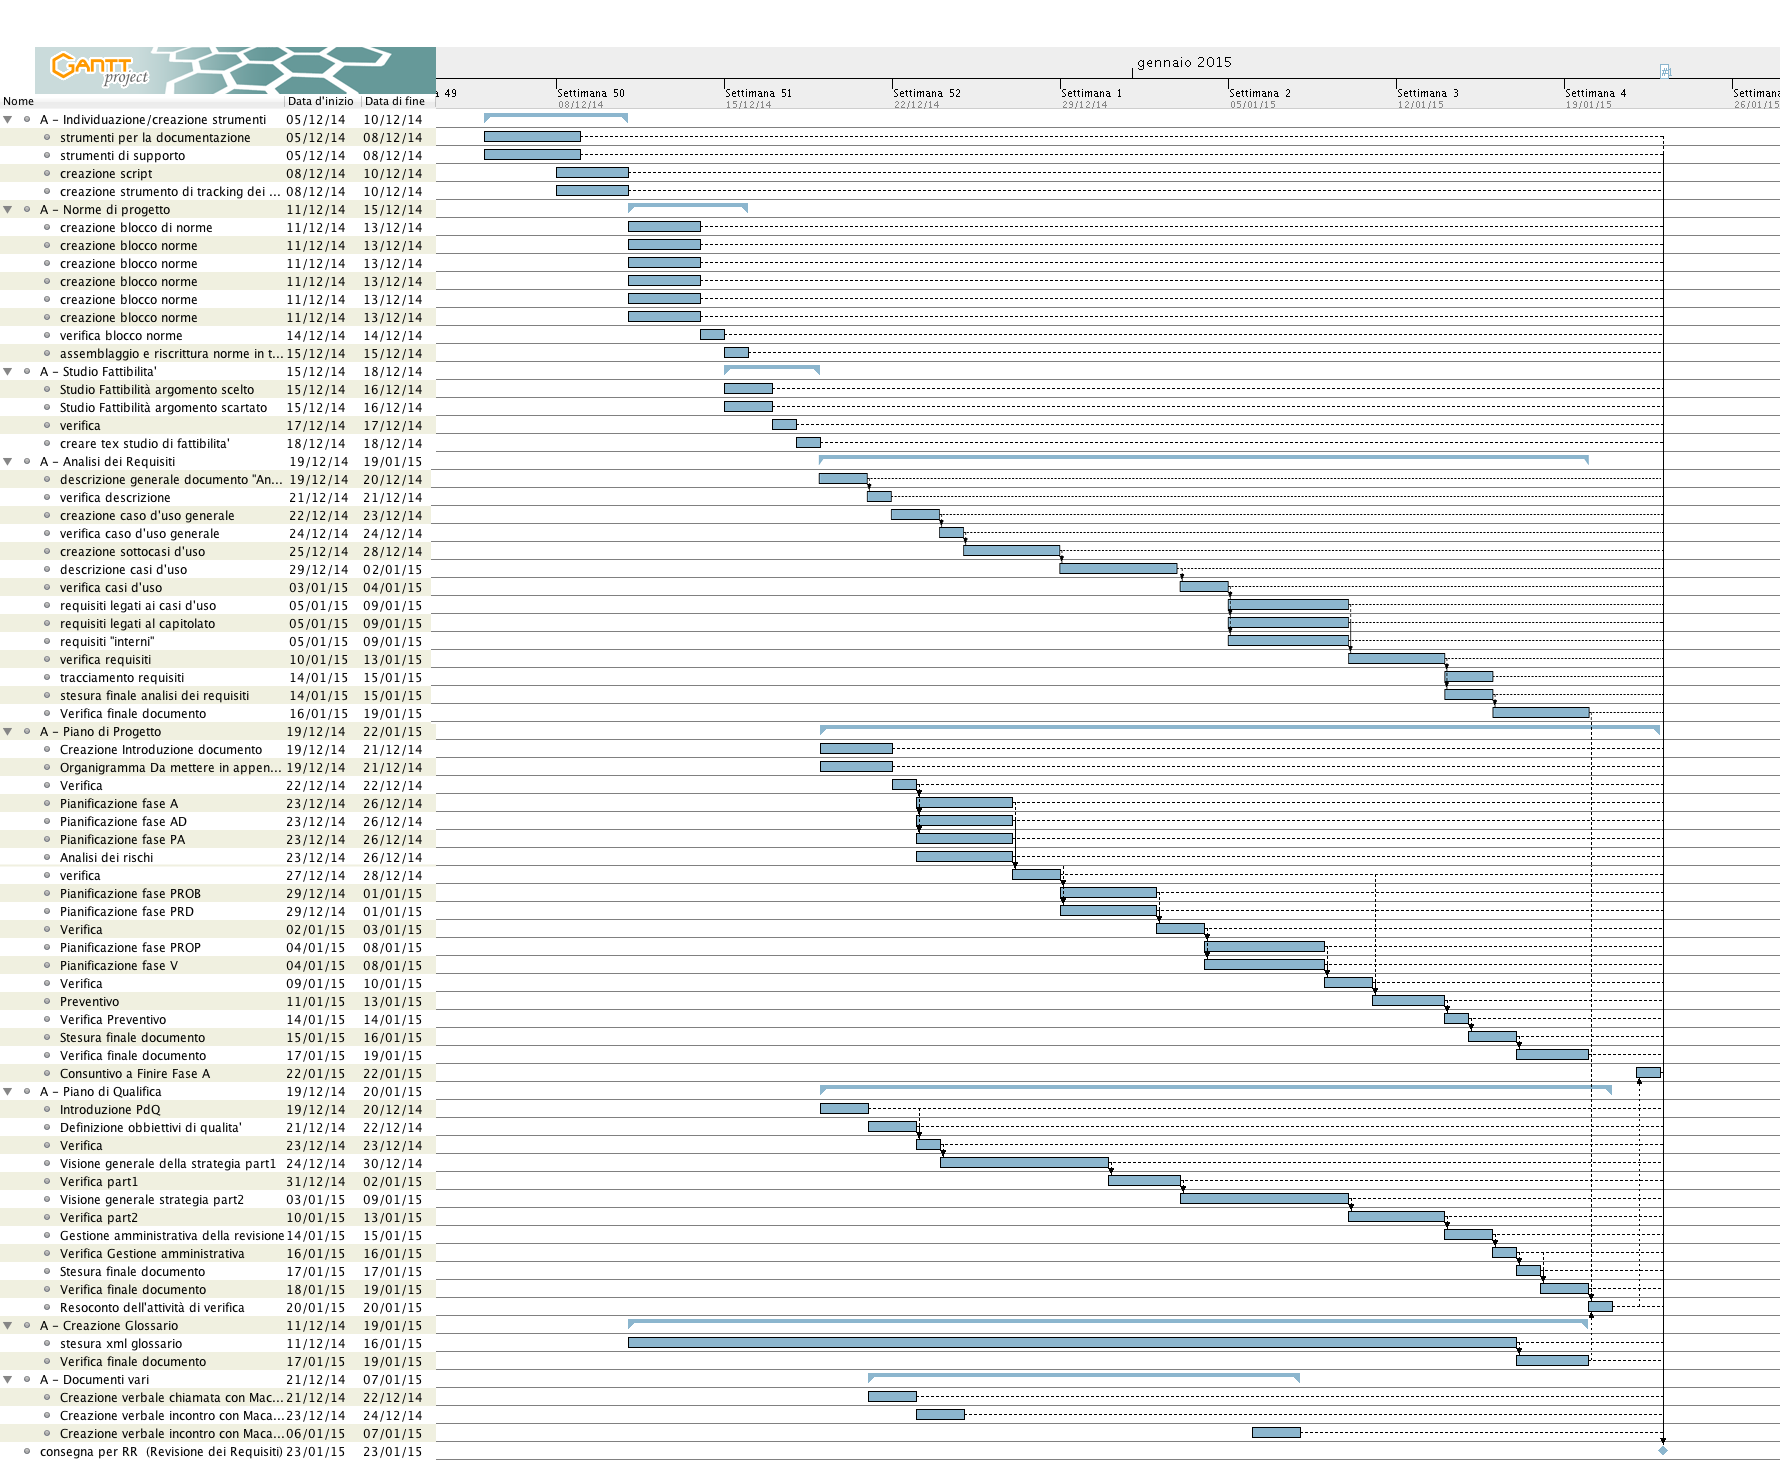
\includegraphics[width=\textwidth]{PianoDiProgetto/Pics/FaseDB.png}
	\caption{Gantt Fase DB}
\end{figure}

	% !TEX encoding = UTF-8 Unicode
\level{3}{Fase DI: Documentation Improvement}
\textbf{Periodo}: dal \insdate{16}{02}{2015} al \insdate{05}{03}{2015} \\
Questa \insglo{fase} comincia al termine della \insphase{Fase DB}. È caratterizzata da una nuova analisi di tutti i documenti redatti nella \insglo{fase} precedente e dalla correzione di questi in base alle richieste e segnalazioni del committente. Gli analisti provvedono, inoltre, all'individuazione di nuovi requisiti e alla correzione di quelli segnalati. Pertanto, i documenti vengono ampliati ed aggiornati alla versione 2.00.
\level{4}{Diagramma di Gantt delle attività}
\begin{center}
	\begin{figure}[H]\centering
		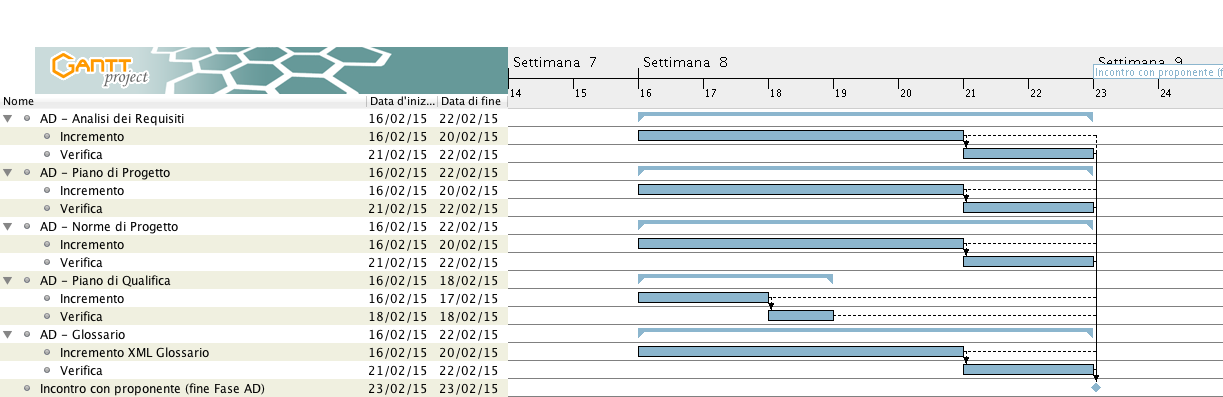
\includegraphics[width=\textwidth]{PianoDiProgetto/Pics/FaseDI.png}
		\caption{Gantt Fase DI}
	\end{figure}
\end{center}

	% !TEX encoding = UTF-8 Unicode
\level{2}{Fase SD: Software Design}
	\textbf{Periodo}: dal \insdate{05}{03}{2015} al \insdate{03}{04}{2015} \\Questa fase comincia con la fine della \insphase{Fase DI} e termina con l'incontro con il proponente per mostrare l'architettura scelta.\\
	Le attività di questa fase sono:
	\begin{itemize}
		\item \textbf{Norme di Progetto}: Viene fatto un incremento alle norme per poter stendere il documento \insdoc{Specifica Tecnica}. Viene successivamente fatta una verifica/validazione per fissare una baseline al documento che diventerà \insdoc{Norme di Progetto v3.00}.
		\item \textbf{Specifica Tecnica}: Questa attività caratterizza la \insphase{Progettazione Architetturale}. Il \insrole{Progettista} stende la \insdoc{Specifica Tecnica} che contiene le scelte progettuali, ad alto livello, che il progetto dovrà avere. Saranno quindi descritti quali design pattern \projectname{} implementerà, l'architettura generale del software, i principali flussi di controllo e il tracciamento dei requisiti.
		\item \textbf{Glossario}: Viene fatto un incremento al Glossario aggiungendo tutti i vocaboli che si ritiene importante siano inclusi. Viene successivamente fatta una verifica/validazione per fissare una baseline al documento che diventerà \insdoc{Glossario v3.00}.
		\item \textbf{Piano di Qualifica}: L'incremento consiste nell'aggiungere al documento \insdoc{Piano di Qualifica v1.00} il dettaglio dell'esito della \insrev{Revisione dei Requisiti} e la parte della pianificazione dei test. Questa attività genererà, dopo una verifica e validazione, il file \insdoc{Piano di Qualifica v3.00}.
		\item \textbf{Piano di Progetto}: l'incremento che sarà fatto al documento \insdoc{Piano di Progetto} in questa fase consiste nell'apportare correzioni nella divisione delle attività e stillare il consuntivo di questo periodo. Dopo un'accurata verifica che fisserà una nuova baseline e la validazione il documento diventerà \insdoc{Piano di Progetto v3.00}.
	\end{itemize}
	\level{3}{Diagramma di Gantt delle attività}
	\begin{figure}[H]\centering
		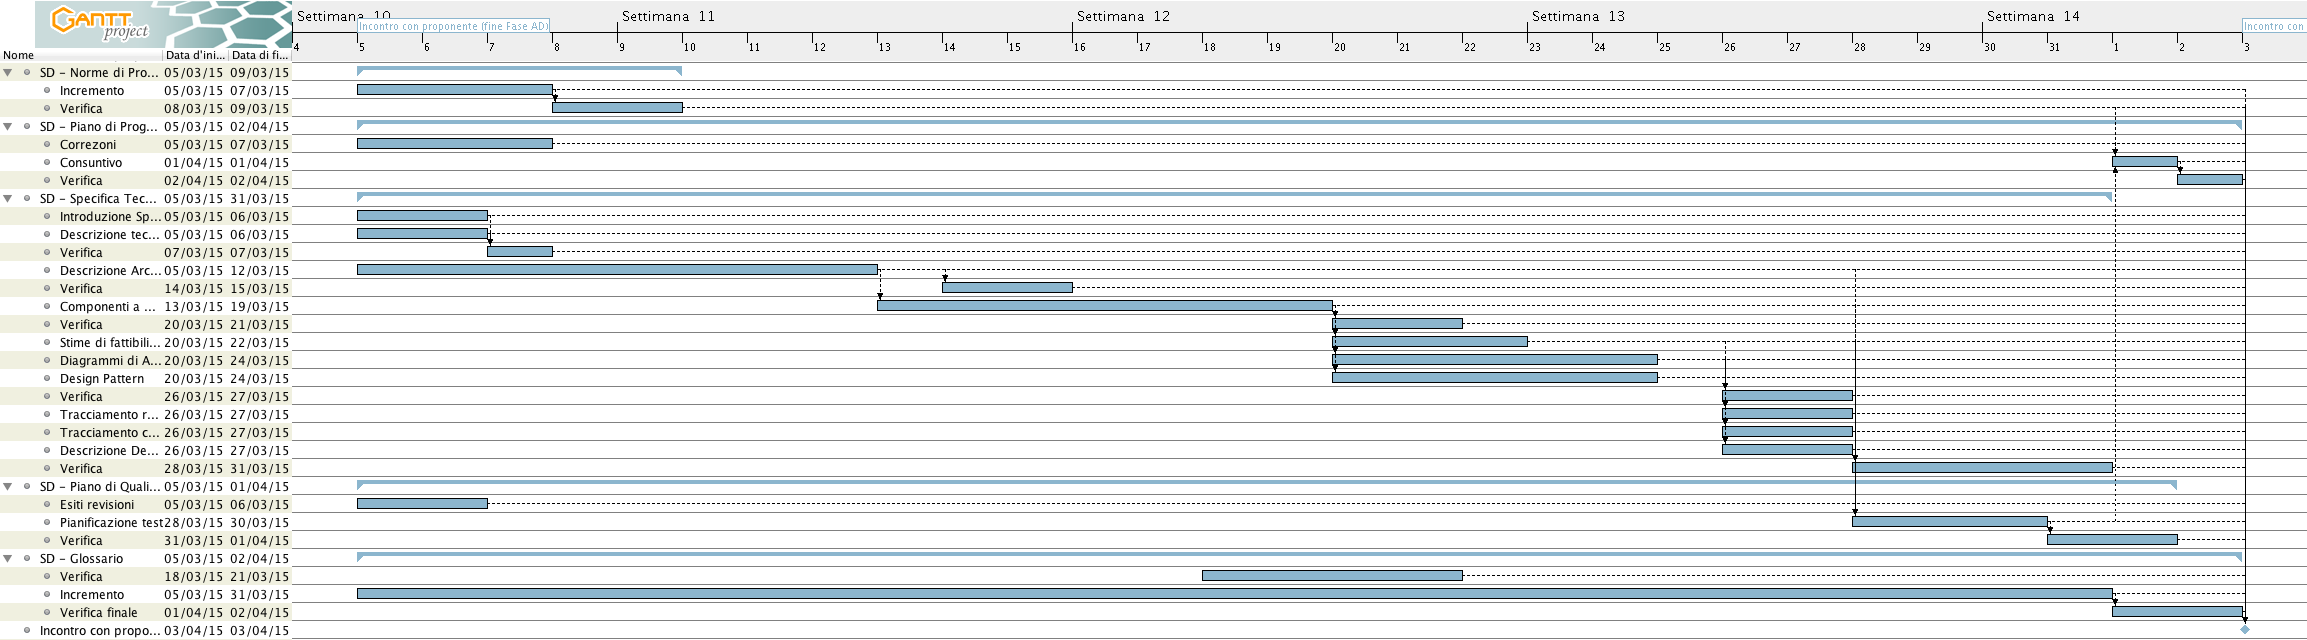
\includegraphics[width=\textwidth]{PianoDiProgetto/Pics/FaseSD.png}
	\caption{Gantt Fase SD}
\end{figure}

	% !TEX encoding = UTF-8 Unicode
\level{2}{Fase P: Prototyping}
	\textbf{Periodo}: dal \insdate{03}{04}{2015} al \insdate{20}{04}{2015} \\Questa fase comincia con la fine della \insphase{Fase SD} e termina con l'incontro con il proponente al fine di mostrare il prototipo con i requisiti obbligatori sviluppati e la scadenza della consegna per la \insrev{Revisione di Progettazione}.\\Le attività di questa fase saranno le seguenti:
	\begin{itemize}
		\item\textbf{Definizione di Prodotto}: viene steso il documento \insdoc{Definizione di Prodotto v1.00}. Esso definisce la struttura interna del sistema e le relazioni dei componenti del prodotto relativi ai requisiti obbligatori.
		\item \textbf{Codifica}: con quest'attività inizia lo sviluppo da parte dei programmatori dei requisiti obbligatori. Sarà dunque seguito quanto riportato nel documento \insdoc{Definizione di Prodotto v1.00};
		\item \textbf{Esecuzione test}: verranno eseguiti automaticamente tutti i test di unità previsti dal documento \insdoc{Piano di Qualifica v4.00};
		\item\textbf{Manuale Utente e Manuale Amministratore}: comincia la stesura dei manuali che forniranno indicazioni agli utilizzatori del sistema.
		\item\textbf{Incremento e Verifica Documenti}: vengono eseguite modifiche ai documenti già scritti, se necessario, che passeranno alla versione 4.00.
		\item\textbf{Glossario}: vengono aggiunti al file \insfile{Glossario.xml} i vocaboli dei quali si ritiene necessaria una definizione formale. Alla fine di questa fase viene quindi generato il documento \insdoc{Glossario v4.00}.
	\end{itemize}
	\level{3}{Diagramma di Gantt delle attività}
	\begin{figure}[H]\centering
		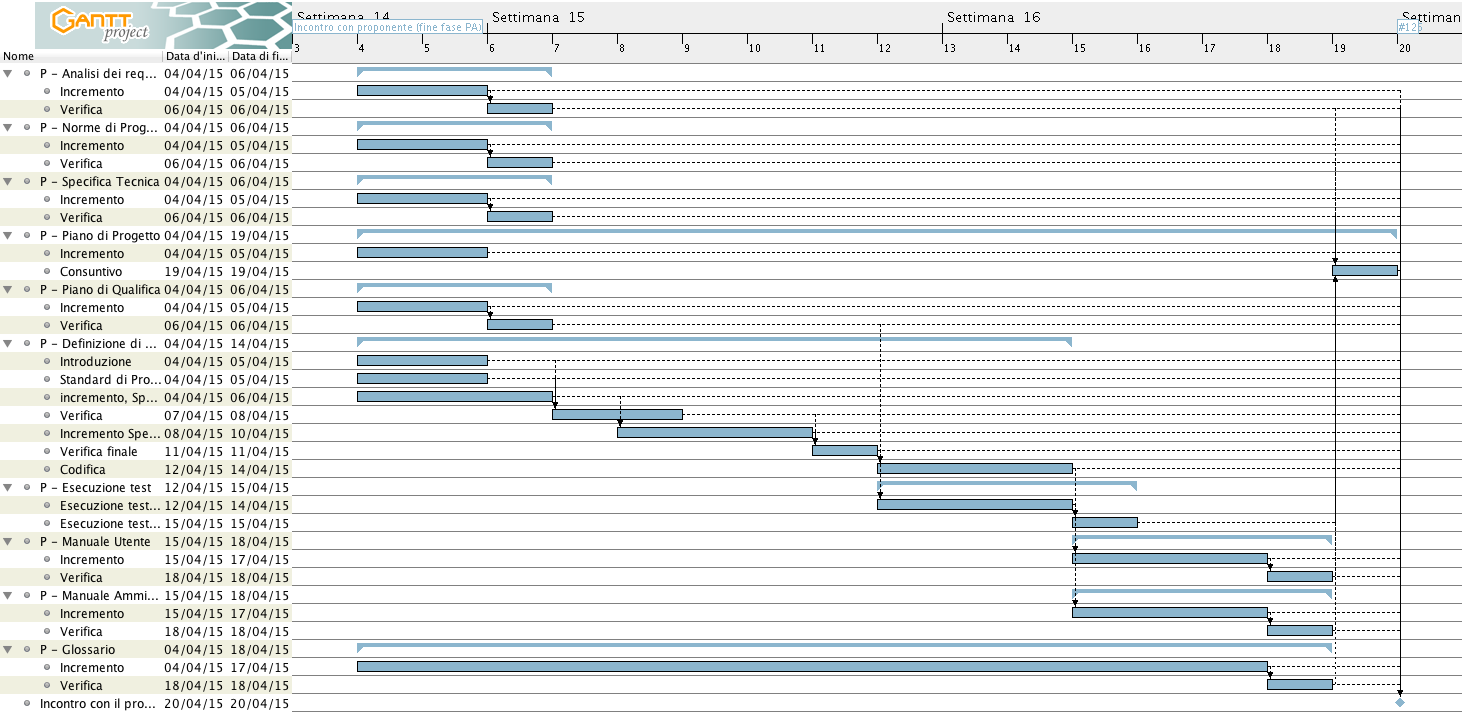
\includegraphics[width=\textwidth]{PianoDiProgetto/Pics/FaseP.png}
	\caption{Gantt Fase P}
\end{figure}
	% !TEX encoding = UTF-8 Unicode
\level{2}{Fase IP: Increase of the Prototype}
	\textbf{Periodo}: dal \insdate{20}{04}{2015} al \insdate{03}{05}{2015} \\Questa fase comincia con la fine della \insphase{Fase P} e termina con la visione del proponente di un secondo prototipo che dovrà soddisfare i requisiti obbligatori e desiderabili. .\\Le attività di questa fase saranno le seguenti:
	\begin{itemize}
		\item\textbf{Definizione di Prodotto}: Viene steso il documento \insdoc{Definizione di Prodotto v2.00}. Esso definisce la struttura interna del sistema e le relazioni dei componenti del prodotto relativi ai requisiti obbligatori e desiderabili.
		\item \textbf{Codifica}: con quest'attività inizia lo sviluppo da parte dei programmatori dei requisiti desiderabili. Sarà dunque seguito quanto riportato nel documento \insdoc{Definizione di Prodotto v2.00};
		\item \textbf{Esecuzione test}: verranno eseguiti automaticamente tutti i test di unità e integrazione previsti dal documento \insdoc{Piano di Qualifica v5.00};
		\item\textbf{Manuale Utente e Manuale Amministratore}: vengono ampliati ed aggiornati i manuali che forniranno indicazioni agli utilizzatori del sistema.
		\item\textbf{Incremento e Verifica Documenti}: Vengono eseguite modifiche ai documenti già scritti, se necessario, che passeranno alla versione 5.00.
		\item\textbf{Glossario}: Vengono aggiunti al file \insfile{Glossario.xml} i vocaboli dei quali si ritiene necessaria una definizione formale. Alla fine di questa fase viene quindi generato il documento \insdoc{Glossario v5.00}.
	\end{itemize}
	\level{3}{Diagramma di Gantt delle attività}
	\begin{figure}[H]\centering
		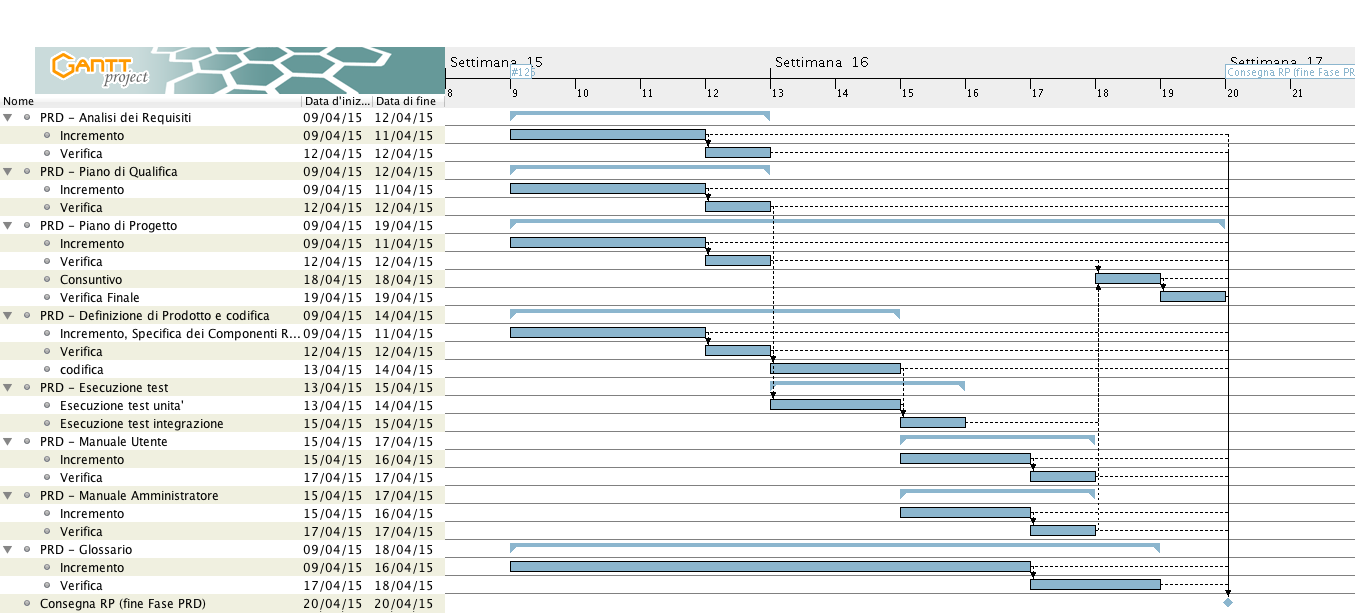
\includegraphics[width=\textwidth]{PianoDiProgetto/Pics/FaseIP.png}
	\caption{Gantt Fase IP}
\end{figure}

	% !TEX encoding = UTF-8 Unicode
\level{2}{Fase CP: Completion of the Product}
	\textbf{Periodo}: dal \insdate{19}{04}{2015} al \insdate{07}{05}{2015} \\Questa fase comincia subito dopo la scadenza della consegna per la \insrev{Revisione di Progetto} e termina con l'incontro con il proponente al fine di mostrare il prototipo con tutti i requisiti (obbligatori, desiderabili e opzionali) sviluppati. 
	\\Le attività di questa fase saranno le seguenti:
	\begin{itemize}
		\item\textbf{Definizione di Prodotto}: viene steso il documento \insdoc{Definizione di Prodotto v3.0}. Esso definisce la struttura interna del sistema e le relazioni dei componenti del prodotto relativi ai requisiti opzionali.
		\item \textbf{Codifica}: con quest'attività inizia lo sviluppo da parte dei programmatori dei requisiti opzionali. Sarà dunque seguito quanto riportato nel documento \insdoc{Definizione di Prodotto v3.00};
		\item \textbf{Esecuzione test}: verranno eseguiti automaticamente tutti i test di unità e integrazione previsti dal documento \insdoc{Piano di Qualifica v 6.00};
		\item\textbf{Manuale Utente e Manuale Amministratore}: comincia la stesura dei manuali che forniranno indicazioni agli utilizzatori del sistema.
		\item\textbf{Incremento e Verifica Documenti}: vengono eseguite modifiche ai documenti già scritti, se necessario.
		\item\textbf{Glossario}: vengono aggiunti al file \insfile{Glossario.xml} i vocaboli dei quali si ritiene necessaria una definizione formale. Alla fine di questa fase viene quindi generato il documento \insdoc{Glossario v6.00}.
	\end{itemize}
	\level{3}{Diagramma di Gantt delle attività}
	\begin{figure}[H]\centering
		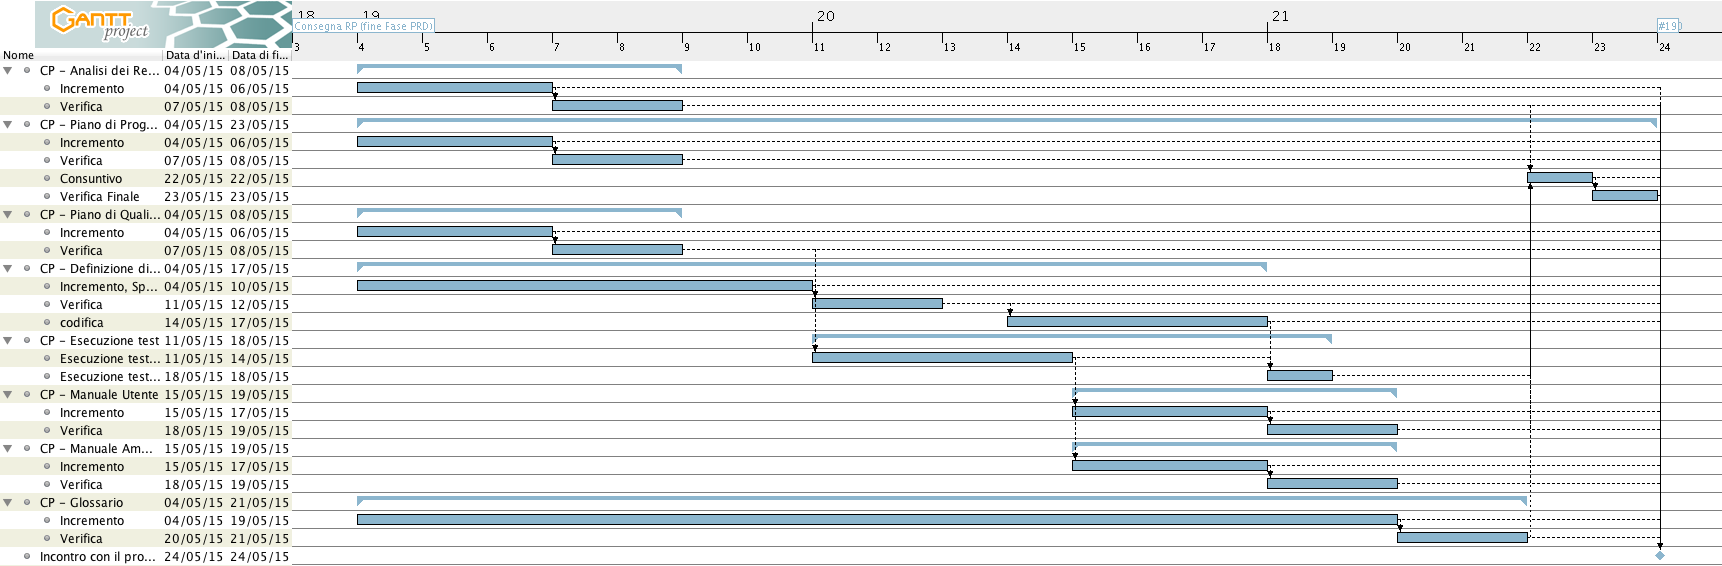
\includegraphics[width=\textwidth]{PianoDiProgetto/Pics/FaseCP.png}
	\caption{Gantt Fase CP}
\end{figure}

	% !TEX encoding = UTF-8 Unicode
\level{2}{Fase PD: Product Delivery}
	\textbf{Periodo}: dal \insdate{28}{05}{2015} al \insdate{17}{06}{2015} \\Questa \insglo{fase} comincia con la fine della \insphase{Fase CP} e termina con la scadenza della consegna per la \insrev{RA}.
	\begin{itemize}
		\item \textbf{Incremento e Verifica}: se necessario verranno effettuati aggiornamenti ai vari documenti scritti, che passeranno alla versione 7.00;
		\item \textbf{Validazione}: viene verificato, attraverso tracciamento, di aver soddisfatto i requisiti presenti nel documento \insdoc{Analisi dei Requisiti v7.00};
		\item \textbf{Esecuzione test}: verranno eseguiti i test di sistema previsti dal documento \insdoc{Piano di Qualifica v7.00};
		\item \textbf{Correzione bug}: i bug rilevati verranno risolti;
		\item \textbf{Collaudo}: viene eseguito e completamente collaudato il sistema creato.
	\end{itemize}
	\level{3}{Diagramma di Gantt delle attività}
		\begin{figure}[H]\centering
			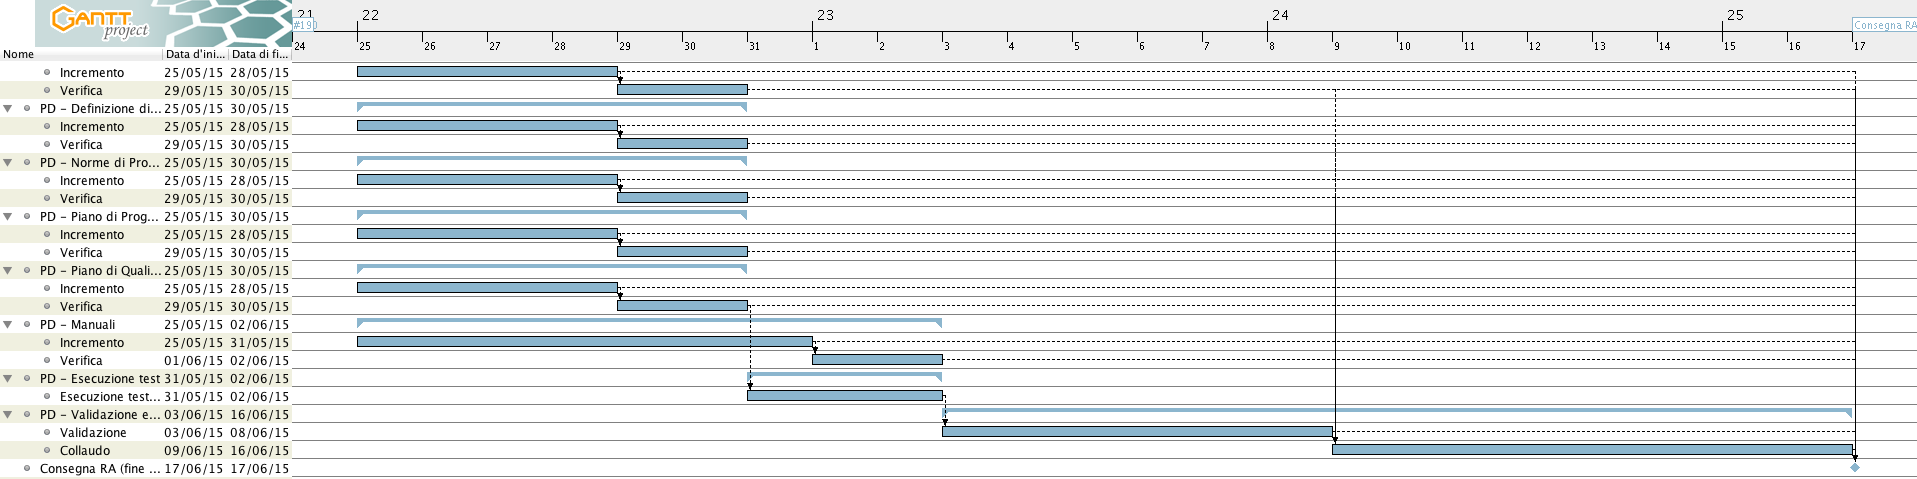
\includegraphics[width=\textwidth]{PianoDiProgetto/Pics/FasePD.png}
		\caption{Gantt Fase PD}
\end{figure}

	
